\documentclass[11pt]{article}

\usepackage[margin=1in, letterpaper]{geometry}
\usepackage{parskip}
\usepackage{amsthm, amsmath, amssymb}
\usepackage{enumerate} % For use of (a), (b), et cetera
\usepackage[pdftex]{graphicx}
\usepackage{hyperref}

% The following metadata will show up in the PDF properties
\hypersetup{
    colorlinks = true,
    urlcolor = black,
    pdfauthor = {Aaron Tran},
    pdfkeywords = {berkeley},
    pdftitle = {Astro 121, UG Radio Lab, Lab 1 - \today},
%   pdfsubject = {},
    pdfpagemode = UseNone
}

% Don't indent paragraphs
\setlength\parindent{0em}

% Problem numbering
\newcounter{iternum}
\setcounter{iternum}{0}
\newcommand{\prob}{\stepcounter{iternum} \textbf{\arabic{iternum}.} }
\newcommand{\probcont}{\textbf{\arabic{iternum}. (cont.) }}

% ===============
% Useful commands
% ===============
\newcommand {\mt}{\mathrm}
\newcommand {\unit}[1]{\; \mt{#1}}
% http://vemod.net/typesetting-units-in-latex

% ==========================
% Document specific commands
% ==========================

\begin{document}

% Titling
\begin{center}
\Large{Design and construction of a $1.045 \unit{MHz}$ FM receiver}

\large
Aaron Tran \\
\today \\
Partners: Patrick Kantorski, Kyle Moses \\
Prof. Aaron Parsons, GSI Karto Keating, uGSI Baylee Bordwell
\end{center}

\section*{\sffamily Abstract}

We present and detail the design of a $1.045 \unit{MHz}$ FM receiver with
bandwidth $200 \unit{kHz}$.  The filter is composed of a bandpass RLC filter,
diode envelope detector, and common-emitter transistor amplifier with gain 2.
Input and output impedances are not matched to appropriate loads or sources but
may be matched by use of emitter-followers or appropriate resistors.  The diode
detector as presented and tested is unusable, but we present a possible
solution as well as an improvement for the common-emitter amplifier.  We
additionally provide a simple procedure to characterize random noise using the
central limit theorem.

% ============
% INTRODUCTION
% ============
\section{Introduction}

Modulation of radio frequency (RF) electromagnetic waves is a simple and
effective method for long distance information transmission, as exemplified by
amplitude/frequency modulated radio.  The generation, transmission, and
reception of modulated signals are interesting engineering problems which are
also accessible to interested amateurs and beginning students of electronics.
Simple modulators and demodulators may be built with a minimum
of passive and active components (i.e., enough to fit on a small breadboard).
RF circuits hold great educational potential for undergraduate students.

Here we present the design and construction of an FM receiver ($1.045
\unit{MHz}$ with bandwidth $200 \unit{kHz}$).  The only non-linear components
necessary are a diode and a transistor.  The primary purpose of this circuit is for self-edification, but the layout may also serve as a starting point for
further exploration of RF circuit design.

The envelope detector as presented is unusable and requires an additional
resistor to ground.  We present simple improvements for the envelope detector
and amplifier, and provide a procedure to characterize receiver noise.

% ==================
% FM RECEIVER DESIGN
% ==================
\section{FM receiver design}

The receiver is comprised of a passive RLC bandpass filter, diode envelope
detector, and a common-emitter amplifier chained between antenna input and
speaker output.  Blocking capacitors between different functional sections
enable voltage biasing.

\begin{figure}[h]
    \centering
    \includegraphics[scale=0.5]{schematics/receiver_box.png} \\
    \textbf{Figure 1.} FM receiver circuit diagram with component values.\\
    Boxes demarcate functional components (see corresponding sections in text).
\end{figure}

\subsection{Bandpass RLC filter}

The input signal is first passed through an RLC filter centered at
approximately $1.045 MHz$ with the $-3 \unit{dB}$ point at $\pm 200 \unit{kHz}$
on each side.  For component values $R, L, C$ (resistor, inductor, capacitor)
and input signal component with angular frequency $\omega$, the gain of this
filter is given by the equation:
\[
  \left| \frac{V_{\mt{out}}}{V_{\mt{in}}} \right| =
    \left[
      1 + (RC)^2 \left(\frac{\omega_0^2 - \omega^2}{\omega}\right)^2
    \right]^{-1/2}
\]
Here $\omega_0 \equiv 1 / \sqrt{LC}$, emphasizing that this filter has unity
gain at $\omega = \omega_0$.  The $-3 \unit{dB}$ roll-off frequency occurs
when the gain is equal to $1/\sqrt{2}$, or when:
\[
  (RC) \frac{\omega_0^2-\omega^2}{\omega} = 1
\]
Let the bandwidth be denoted by $\Delta f$, with corresponding cut-offs at
$f = f_0 \pm \Delta f /2$, where $f_0 = w_0/(2\pi)$.  This gives:
\[
  2 \pi f_0 RC \approx \frac{f_0}{\Delta f}
\]
as a prescription for our cut-off.  Our component values $R = 33 \unit{\Omega},
L = 1 \unit{\mu H}, C = 22 \unit{nF}$ give $f_0 = 1.073 \unit{MHz}$ with
bandwidth $\Delta f = 220 \unit{kHz}$.  Figure 2 plots the frequency-dependent
gain along with the transmission band of interest at $1.045 \unit{MHz}$.

\begin{figure}[h]
    \centering
    \includegraphics[scale=0.4]{scripts/rlc_filter_gain.pdf} \\
    \textbf{Figure 2.} RLC filter gain against input frequency $f$ (Hz).\\
    FM signal bandwidth plotted in light green.
\end{figure}

\subsection{Diode envelope detector}

We use a diode in series with a low-pass RC filter as a rudimentary envelope
detector.  Prior to a diode, we use a blocking capacitor and voltage divider to
apply a bias voltage of $0.68 \unit{V}$ to the input signal; this allows the
positive half of the signal to be passed mostly unattenuated by the diode.

The blocking capacitor value is set by the behavior of the capacitor and the
biasing voltage divider as a high pass filter.  Looking into the voltage
divider, the resistors are seen in parallel and so the input impedance is
about $860 \unit{\Omega}$.  To allow our carrier signal ($\sim 1 \unit{MHz}$)
to pass, the blocking capacitance must be at least $0.2 \unit{nF}$,
which is satisfied by our $1 \unit{\mu F}$ capacitor.

Our diode circuit is expected to obtain a signal envelope as follows.  The
diode extracts only the positive half of an input signal, with the diode's knee
voltage compensated for by our voltage biasing.  However, when the carrier
signal peaks and begins to decrease, the RC circuit prevents the maximum
imposed voltage from decaying immediately; it is forced to decrease over a
timescale $RC$.  The voltage is only ``unpinned'' once the next carrier cycle
passes through the diode.

The diode is placed in series with a low-pass RC filter of cutoff frequency
$\sim 110 \unit{kHz}$.  In actuality, the cutoff frequency should have been
closer to $1 \unit{MHz}$ for envelope detection.  Our envelope
detector did not operate correctly anyways, which we discuss further below.
We plot the gain of the low-pass filter in Figure 3, to show that audible
frequencies will not be attenuated in a correctly designed circuit.

\begin{figure}[h]
    \centering
    \includegraphics[scale=0.4]{scripts/diode_rc_lowpass_gain.pdf} \\
    \textbf{Figure 3.} Low-pass RC filter gain as a function of input frequency
    $f$ (Hz).  Approximate human hearing range plotted in light green.
\end{figure}

\subsection{Common-emitter amplifier}

We pass the extracted envelope curve from the diode demodulator to a
common-emitter transistor amplifier.  Our choice of component values and
following explanation of circuit operation are guided in large part by
\emph{Horowitz and Hill} [1989].

The transistor's quiescent base voltage is set by a biasing voltage divider,
which controls emitter voltage.  For appropriate choice of collector and
emitter resistors, the collector voltage amplifies the base voltage signal.
The gain is given as $-R_c / R_e$ (where $R_c$, $R_e$ denote collector and
emitter resistors respectively).

For maximal voltage swing, the quiescent collector voltage should be
$2.5 \unit{V}$ (or, $V_{\mt{cc}}/2$).  We choose a quiescent current of
$1 \unit{mA}$ and hence set collector resistor to $2.5 \unit{k\Omega}$.  We set
the emitter resistor at $1.25 \unit{k\Omega}$ for a gain of $2$. The quiescent
emitter voltage is then $1.25 \unit{V}$, and the quiescent base voltage
should be $\sim 1.85 \unit{V}$.  We bias the base voltage using
$22 \unit{k\Omega}$ and $13 \unit{k\Omega}$ resistors.

In actual practice, we used slightly different values ($R_E = 1.5
\unit{k\Omega}$, $R_C = 2.7 \unit{k\Omega}$, voltage divider resistors $22
\unit{k\Omega}$ and $12 \unit{k\Omega}$).  However, our results are not
significantly affected.

The blocking capacitor prior to the amplifier biasing circuit acts as a
high-pass filter.  The input impedance, looking into the transistor
base, is $\sim 8 \unit{k\Omega}$ (set primarily by the two divider resistors
in parallel).  We choose $0.68 \unit{\mu F}$ as our capacitor, which gives a
cut-off frequency of $30 \unit{Hz}$, at the lower end of the audible range
(cf. Figure 3).

\subsection{Receiver impedances}

External loads or sources (antennae, transmission lines, speakers) connected to
our receiver should be impedance matched to maximize power throughput.

The output impedance of the amplifier sets the receiver's output impedance, as
the amplifier transistor buffers any lower impedance upstream.  In our circuit,
the output impedance is the parallel impedance of the transistor and collector
resistor, or roughly $2.5 \unit{k\Omega}$.  This is much larger than the $50
\unit{\Omega}$ impedance of transmission lines, or the $8 \unit{\Omega}$
impedance of our speaker.

An emitter-follower circuit may be placed after the amplifier, then, to
decrease the receiver's output impedance by a factor of $\sim 1/\beta$; $\beta$
is the transistor amplification factor.  We may make further adjustments by
placing resistors in parallel with the follower output, or adding resistors in
series with the speaker at the end of the line (although, I'm not sure what is
common practice).

The input impedance appears more difficult to calculate.  For signals far from
the bandpass, the LC tank circuit provides a low-impedance path to ground; for
signals within the bandpass (i.e., where the tank circuit is resonant and
impedes flow to ground), we would have to consider the impedance of our diode
circuit.

% =======
% RESULTS
% =======
\section{Results}

To test the RLC bandpass filter, we input a sine wave of varying frequencies
and measured the output across the $LC$ tank circuit.  We obtained a maximum
gain of $0.83$ at input frequency $1.05 \unit{MHz}$ (caveat: we may have used
incorrect termination procedure for this measurement, but this only impacts our
gain measurement).  The circuit qualitatively showed the correct roll-off
behavior.

When we input an FM signal at $1.045 \unit{MHz}$ and observed the
filter output on an oscilloscope, the signal was correctly converted into
an AM signal with envelope code matching output audio.  We also confirmed that
the voltage divider added a bias of approximately $0.7 \unit{V}$.
However, the diode envelope detector appeared to flatline and output a roughly
fixed voltage.

When testing the demodulator circuit, with or without amplifier, the speaker
appeared to output audio when connected to the circuit output.  However, we
found that the audio level was independent of whether the circuit was powered,
or whether the FM signal was even connected to the circuit input.

The common-emitter amplifier begins clipping at input of
$1.4 \unit{V_{\mt{pp}}}$; this corresponded to output
$2.34 \unit{V_{\mt{pp}}}$.  At this input, there appeared to be a very small
voltage difference between collector and emitter.
For smaller voltages at $10 \unit{kHz}$ it functioned correctly.

% ==========
% DISCUSSION
% ==========
\section{Discussion}

\subsection{Envelope detector design}

The fatal flaw in our envelope detector is, simply, that there is no path to
ground. After a cycle maximum, the voltage at the back of the diode decreases,
but the voltage at the front of the diode is held constant by the filter and
blocking capacitors, which can only discharge through diode leakage current at
sufficiently low input frequencies.

The traditional resolution to this problem is to neglect the series resistor
(in the low-pass RC filter) and instead place a resistor in parallel to ground.
As before, the characteristic time $RC$ should be comparable with the timescale
of carrier wave oscillations (i.e., $1 / (1 \unit{MHz})$).  Unfortunately, we
neglected this and so our circuit design is inoperable.

\subsection{Common-emitter amplifier design}

Without the bypass capacitor, the amplifier frequency bounds are set by 1. high
pass filter of blocking capacitor and bias divider, and 2. stray circuit and/or
transistor capacitance.  We did not collect measurements to characterize
frequency dependence of amplification in our actual circuit, however.

Although effective, the amplifier design presented can only tolerate so much
gain.  As the emitter resistor is made smaller, the current flow is
increasingly influenced by the temperature dependent transistor resistance
($r_e$), as described by the transconductance model [\textit{Horowitz and
Hill}, 1989]. The biasing circuit exerts less control on the emitter voltage
and so the circuit is less reliable.

Both gain and stability may be improved by adding an emitter capacitor ($C_e$)
in parallel with the resistor capacitor.  The new gain is:
\[
  \left| \frac{V_\mt{out}}{V_\mt{in}} \right|
    = \left[ \left(\frac{R_c}{R_e}\right)^2
      + \omega^2 R_c^2 C_e^2 \right]^{1/2}
\]
By choosing $C_e = 50 \unit{nF}$, we were able to observe 10x gain at input
frequency $10 \unit{kHz}$.  However, the gain with capacitor preferentially
amplifies higher frequencies, and we have neglected transistor resistance
$r_e$.

We may address both issues by placing an emitter resistor in series with a
bypassed emitter resistor (Figure 4).  The following analysis, again, is
largely informed by \textit{Horowitz and Hill} [1989].

\begin{figure}[h]
    \centering
    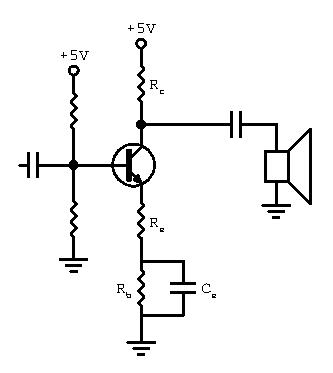
\includegraphics[scale=1]{schematics/amplifier_bypass.pdf} \\
    \textbf{Figure 4.} Circuit schematic of common-emitter amplifier \\
    with partially-bypassed emitter resistor.
\end{figure}

The gain of this circuit (not bothering to take an absolute value) is
\[
  \frac{V_\mt{out}}{V_\mt{in}}
    = \frac{R_c} { R_e + (R_b)/(1+j\omega R_b C_e) }
\]
where $j$ is the imaginary unit, and we have denoted the bypassed resistor by
$R_b$.  We have neglected transistor resistance $r_e$, which may be included
via $R_e$ if desired.  For sufficiently large $\omega$, the
term $R_b/(1+j\omega R_e C_e)$ becomes unimportant and the gain reduces to
$R_c / R_e$.  However, the quiescent voltage is set by $R_e + R_b$, which
improves stability (e.g., reduces likelihood of current saturation).

To obtain a stable gain over the frequency band of interest, we need only
consider the lowest frequency $\omega_{\mt{min}}$ and impose the condition
\[
  \frac{R_b^2}{1 + \omega_{\mt{min}}^2 R_b^2 C_e^2} << R_e^2
\]
For $R_c = 2.5 \unit{k\Omega}$ and $\omega_{\mt{min}} = 20 \unit{Hz}$, we might
pick $R_e = 250$, $R_b = 1 \unit{k\Omega}$ and $C_e = 32 \unit{\mu F}$.  This
would give a stable gain of $10$ for all frequencies above $\sim 20 \unit{Hz}$.

\subsection{Noise simulation and characterization}

We attempted to quantify the Johnson-Nyquist noise in a resistor and in our
receiver by using two amplifier stages, each with gain $24.5 \unit{dB}$ at
frequencies below $1.2 \unit{GHz}$.  In the process, we discovered that a
majority of available commercial amplifiers were dysfunctional and that we
could not obtain any amplification.  Nevertheless, we present some theoretical
calculations, simulations, and a procedure for estimating the noise figure of
our receiver.



Blah amplifiers, bandwidth and Johnson-Nyquist noise, oscilloscope noise.

Thermal noise, resistor.


* Amplifier test - explain Allan variance test, but give reasonable physical numbers

\section{Conclusion}

What you're gonna do with this next.  Don't rewrite your intro/abstract.

Use plain english.  Don't worry about being technical, or too concise...

We are missing a substantial number of error estimates (usually numbers are
good to the last digit, maybe $\pm 2 or 4$ in that least significant digit).
And, we did not take many measurements to gauge our circuits' frequency
responses in actual operation.

\section{Acknowledgments}

Thanks to Patrick and Kyle for much patience and time in lab.  Much thanks to
Baylee, Karto, and Prof. Parsons for answering our questions and helping us
root out some mistakes (though not all, as evidenced here).  Other lab members
are thanked for discussions of variable seriousness and positive utility.

\section{References}

\hangindent 0.25in Horowitz, P. and W. Hill (1989), \emph{The Art of
Electronics}, Cambridge Univ. Press, Cambridge, UK.

\end{document}
